

\chapter{\texorpdfstring{The hardness of the \ce{Ti2Ni} structure}{The hardness of the Ti2Ni structure}}
\graphicspath{{hardness_of_ti_2_ni/Figs/}}
\label{chap:ti2ni_hardness}



The previous chapters have explained previous observations about dislocations in almost ideal model systems, alkali halides and the MAX phases, but are the models of dislocation motion in those materials applicable more broadly, hopefully with a greater applicability to industrial problems. A candidate system should fit some criteria: The MAX phases can accommodate chemically and hence elastically heterogeneous regions because the unit cells are large, at least in the $c$ axis along which the heterogeneity is greatest, so the unit cell of any candidate must be large, of the order of \SI{10}{\angstrom}. The MAX phases show very easy slip in the basal plane, but slip out of that plane is much harder, so ideally any candidate phase will have higher crystal symmetry, certainly cubic, and with enough independent slip systems to allow full plasticity. The MAX phases also allow a large range of heterogeneity to be investigated due to the wide range of stable compositions, so a range of alloying possibilities is required.

The \ce{Ti2Ni} structure was selected because it meets all of these criteria to an adequate extent. The structure is an FCC crystal structure with 96 atoms in the unit cell and, for the case of titanium and nickel, a lattice parameter of \SI{11.28}{\angstrom} \cite{Yurko1959,Yurko1962}. The range of elements that can be incorporated into the structure is also large, a search using the Inorganic Crystal Structure database \cite{ICSD} returned 103 results including elements such as sodium,  zinc, germanium, niobium and hafnium, amongst others.

\section{The \texorpdfstring{\ce{Ti2Ni}}{Ti2Ni} structure}
\FloatBarrier


Phases with the \ce{Ti2Ni} structure is a large unit cell with a large number of atoms and appears complex, a plan view is shown in \autoref{fig:Ti2Ni_plan}. However the symmetry of the structure is high, the space group is Fd\={3}m, and there are only three symmetrically distinct sites; the wyckoff positions for which are 16(c) (Ti1), 32(e) (Ni) and 48(f) (Ti2), which have the coordination numbers 12, 12 and 14 respectively. The ordering of these clusters creates the face-centred symmetry. The creation of a face-centred structure, rather than an icosahedral packing, requires distorted icosahedral coordination polyhedra.


\begin{figure}[h]
\centering
\includegraphics[width=0.5\textwidth]{Ti2Ni_structure}
\caption{Plan view of the \ce{Ti2Ni} structure down the [001]. The blue atoms are titanium sites and the silver atoms are nickel sites.\label{fig:Ti2Ni_plan}}
\end{figure}



While in many phases descriptions of structures the clusters are little more than geometrically elucidating \cite{Steurer2006}, in the \ce{Ti2Ni} phases there is direct evidence that the bonding and properties are highly localised into the clusters, particularly the 16(c) site, at which a titanium atom sits \cite{Ivanovic2006}. \citet{Ivanovic2006} examined the electric field gradient of the material and found it to be extremely heterogeneous, showing different bonding at the two titanium sites, the 16(c) and the 48(f), just \SI{3}{\angstrom} apart. The 16(c) coordination cluster is found to be the most stable and to have a metallic character to its bonding. The cluster at the 32(e) site is less stable but has otherwise similar character to the coordination cluster at 16(c), appearing in both the \ce{Ti2Ni} structure and in a related quasicrystal imply this is a natural complement to the 16(c) cluster, i.e. the two arrangements pack well. The 48(f) arises in the crystalline state but not the quasicrystalline state, and so must be a product of space filling in the \ce{Ti2Ni} crystal structure. The 48(f) cluster shows a large variation bond lengths among bonds of the same type; \citet{Ivanovic2006} ascribe this to a covalent character in the bonding.


The details of the bonding are not of primary interest however, rather it is in how this might relate to dislocation motion. Here we must consider not clusters but broader regions of crystals. If the clusters are physically significant structural units then the way these pack together will be key to the dislocation properties, just as in close-packed metals the way atoms pack together is key to the character of dislocations in simple metals. The 16(c) sites form chains, sharing faces and definin a tetrahedron within the unit cell. This is in fact a Kagom\'{e} net, exactly as exists in the Laves phases \cite{Stein2004,Stein2005}, which are planes parallel to the \{111\} planes. This network is shown in \autoref{fig:16c_network_Ti2Ni}

\begin{figure}
\centering
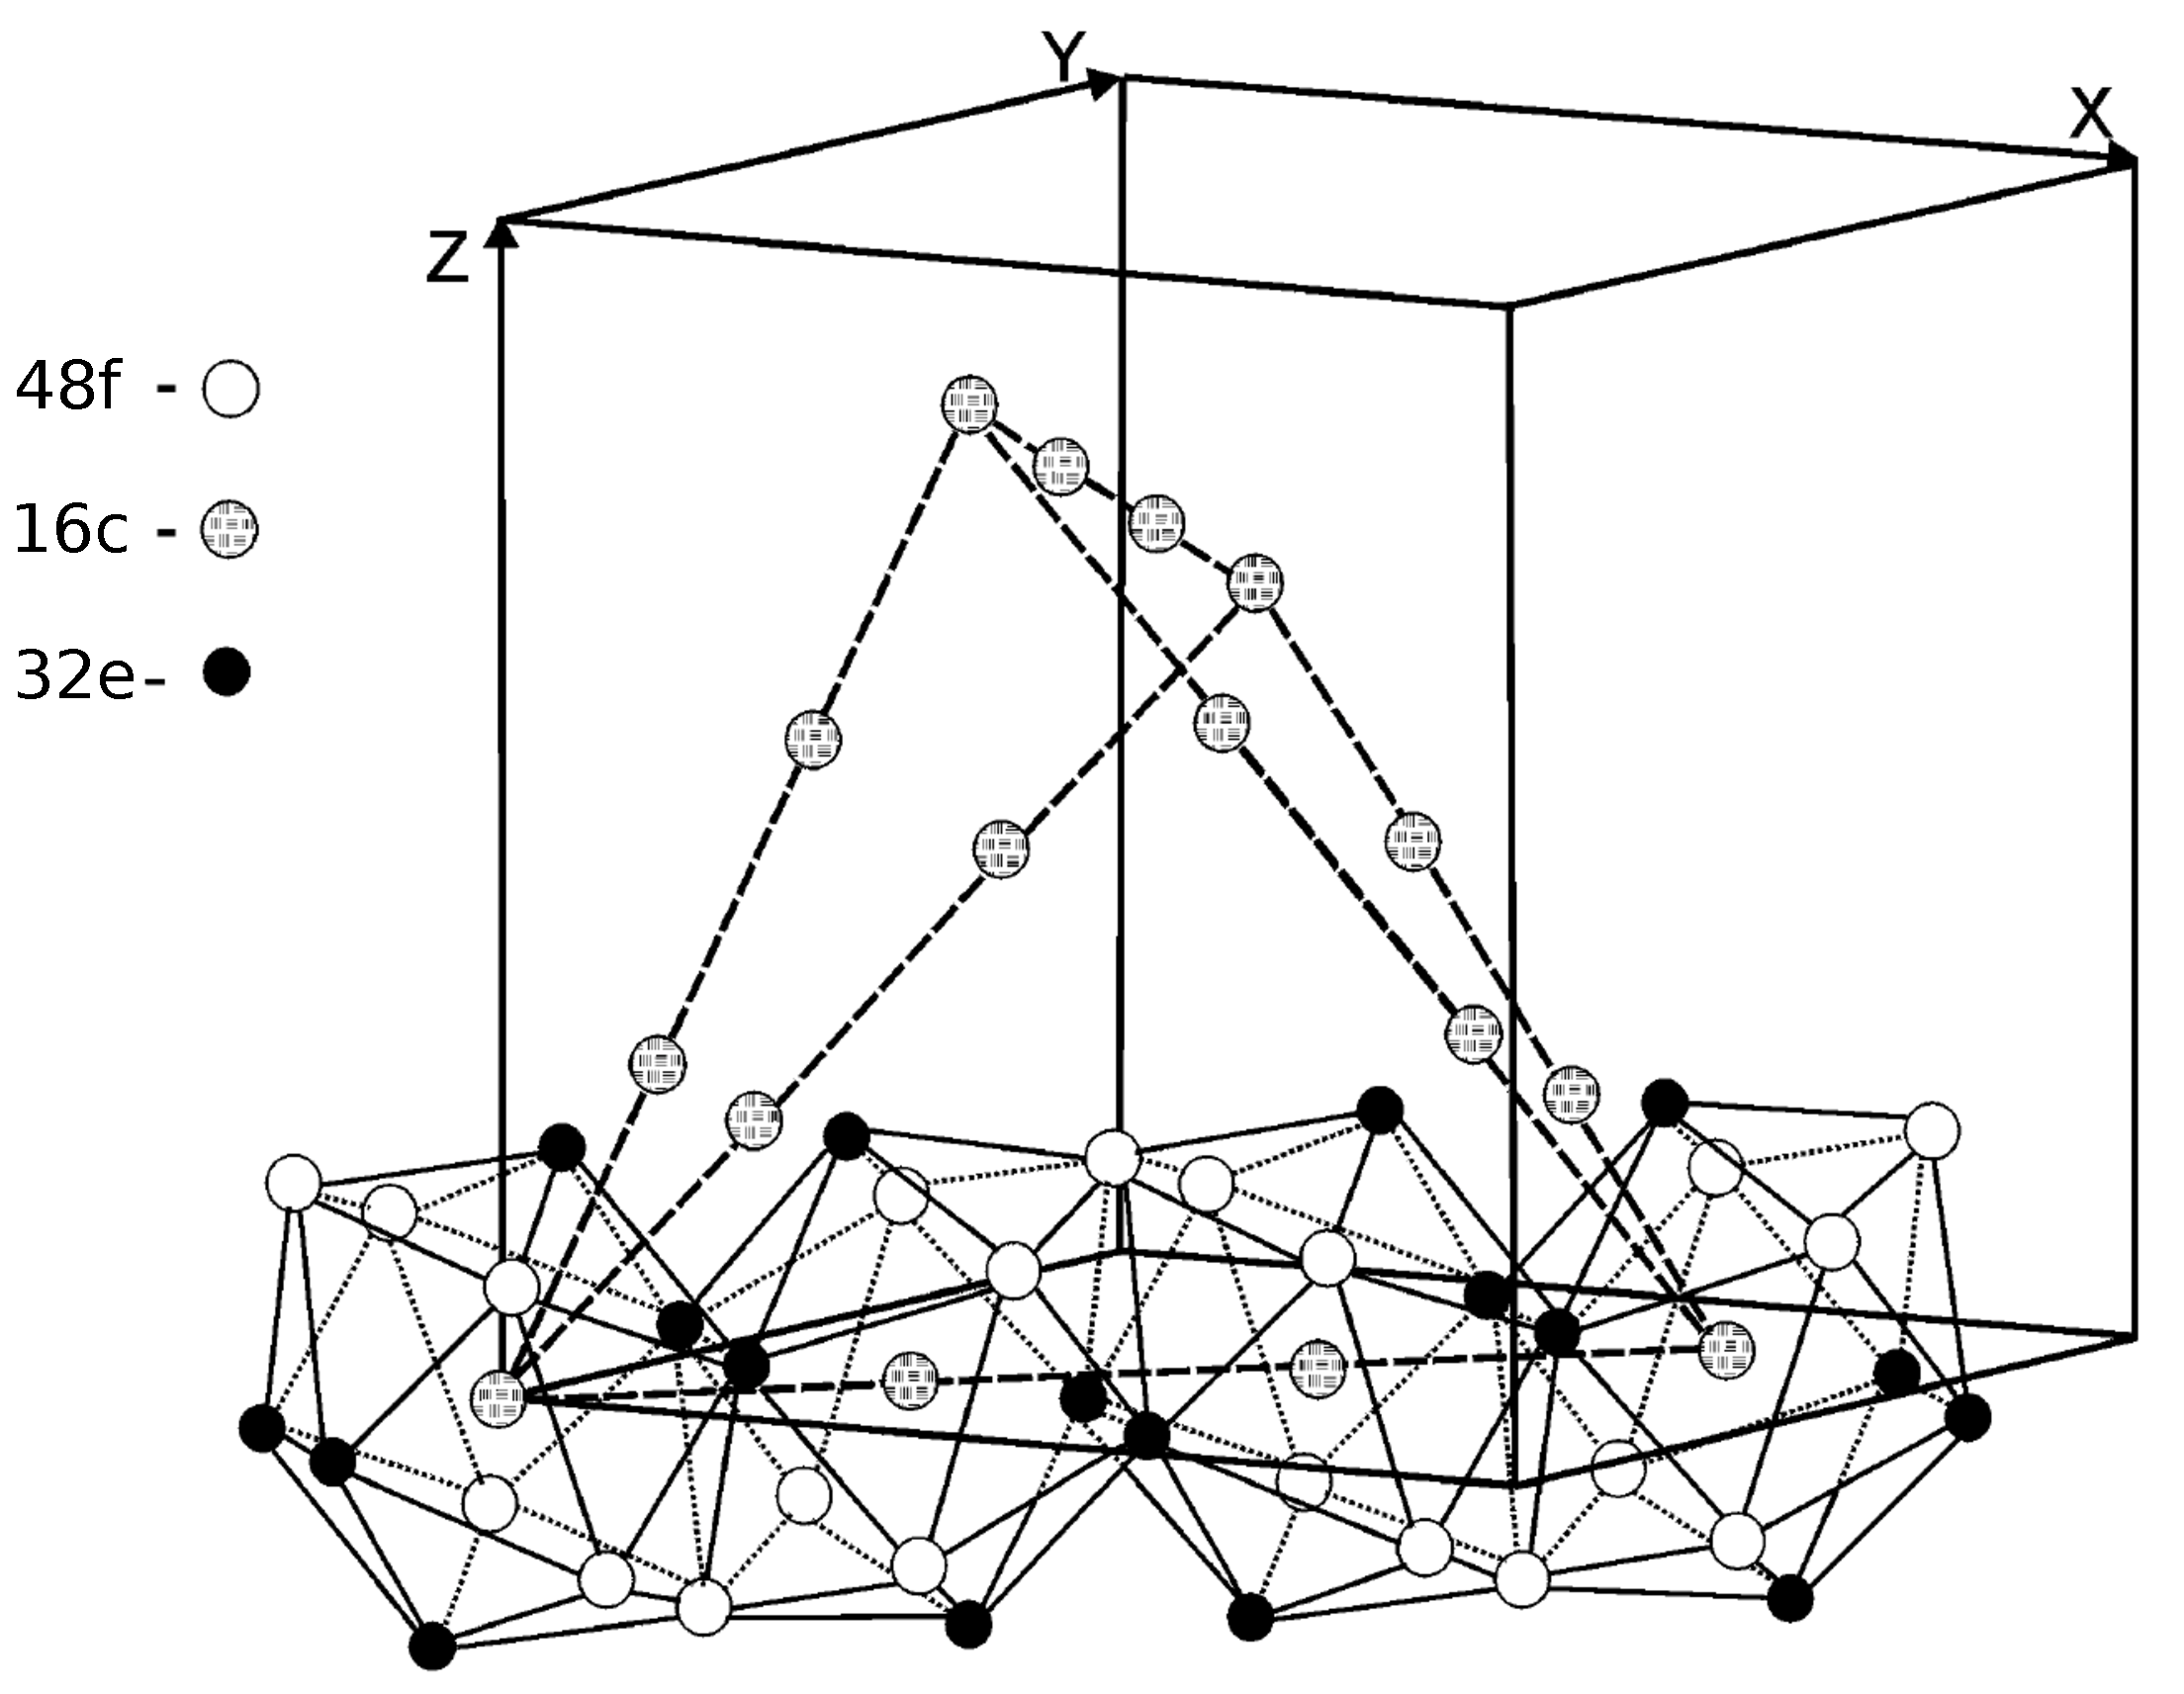
\includegraphics[width=0.5\textwidth]{Ti2Ni_16c_sites}
\caption{The network formed by the metallically bonded coordination clusters at the 16(c) site in the \ce{Ti2Ni} structure, reproduced from \cite{Ivanovic2006}.\label{fig:16c_network_Ti2Ni}}
\end{figure}


Dislocations are long, linear defects and so will respond to the properties of extended regions of a crystal. In other face-centred cubic intermetallics with large unit cells slip has been shown to be on the \{111\} planes and in either <1\={1}0> or <11\={2}> directions, in a simple analogy with FCC metals \cite{Davis2015}. The \{111\} planes are shown in \autoref{fig:Ti2Ni_111_planes}. It is clear that the heterogeneity inherent in the crystal is relevant to the slip system that is likely to operate in this structure since there are distinct layers in the structure when viewed in this way. The view in \autoref{fig:Laves_phase_Ti2Ni_similarity} shows a marked similarity with the Laves phase structure which similarly has a Kagom\'{e} layer and a puckered triple layer, albeit with shorter repeat distances. An important point is that it seems reasonable to take the Kagom\'{e} layer to be formed by the 16(c) clusters, in which case the network of intersecting Kagom\'e layers contains all the nickel sites, 32(e), in the crystal, an the space between is filled by titanium atoms on the 48(f) site.


\begin{figure}
\centering
\begin{subfigure}{0.65\textwidth}
\centering
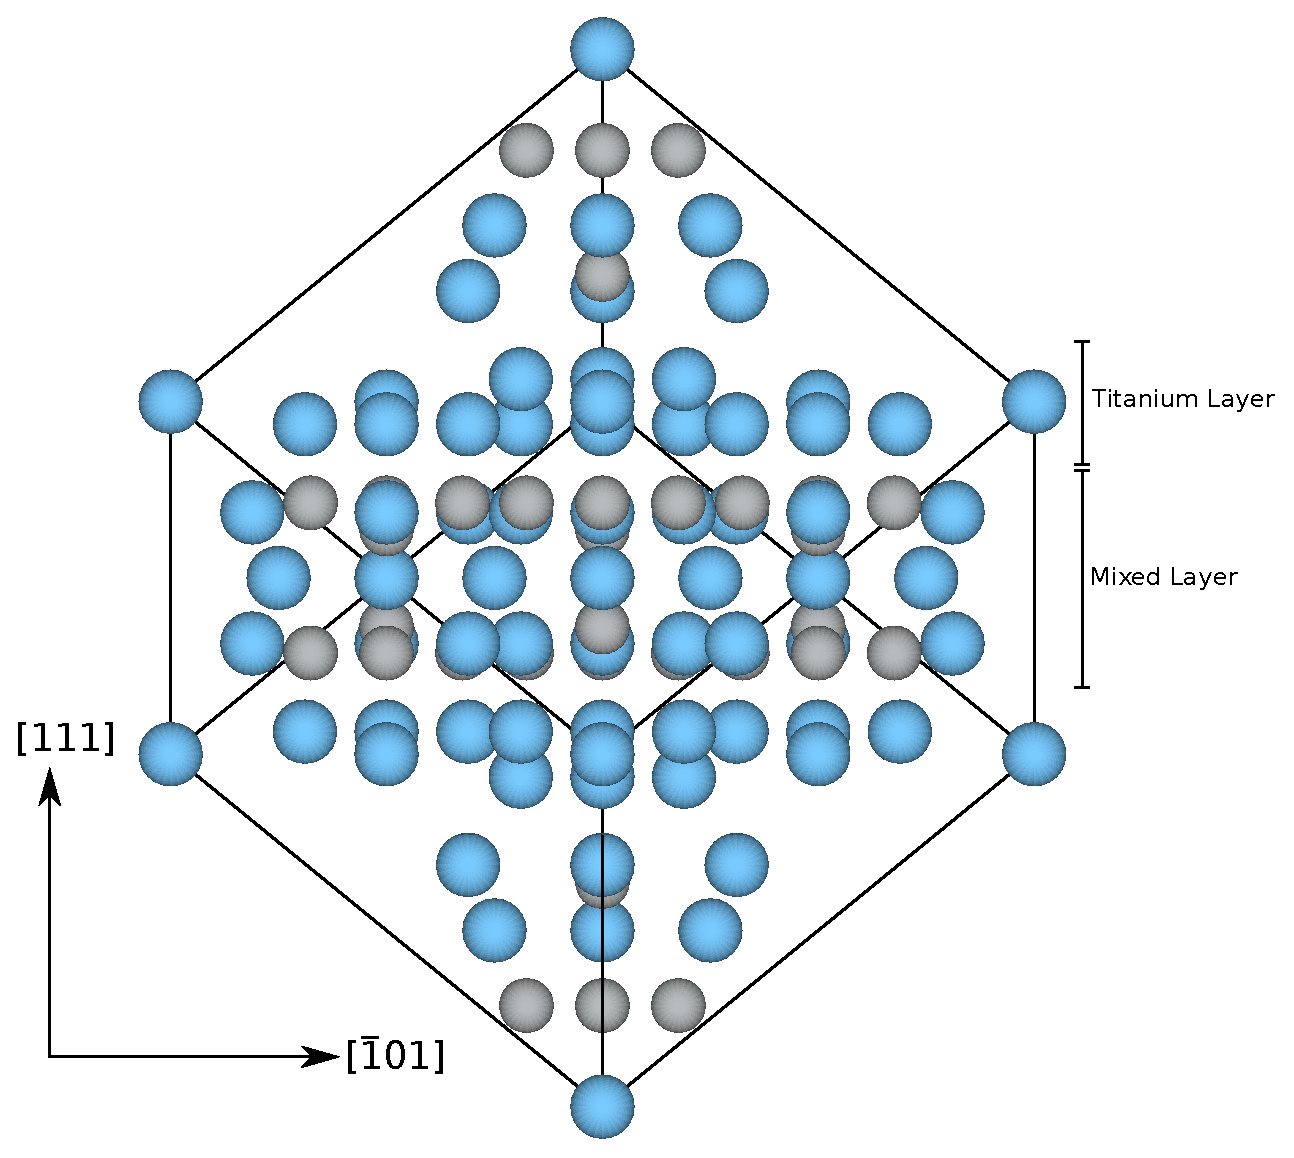
\includegraphics[width=\textwidth]{Ti2Ni-slip_system}
\caption{A view of the \ce{Ti2Ni} unit cell showing the \{111\} planes with the ``ideal'' burgers vector across the diagram.\label{fig:slip_system_Ti2Ni}}
\end{subfigure}

\begin{subfigure}{0.65\textwidth}
\centering
\includegraphics[width=\textwidth]{Ti2Ni-layers}
\caption{A view of the \ce{Ti2Ni} structure showing the \{111\} planes looking down the <\=101> direction.\label{fig:Laves_phase_Ti2Ni_similarity}}
\end{subfigure}
\caption{The \{111\} layers of the \ce{Ti2Ni} structure projected along two different directions.\label{fig:Ti2Ni_111_planes}}
\end{figure}

\subsection{The alloying additions and effects}

To assess the effect of alloying additions on the dislocations salient regions of the crystal structure must be considered, at least to a degree; plainly the situation for \ce{Ti2Ni} is not as simple and clear cut as the MAX phases considered in \autoref{chap:dislocations_in_max_phases}, which have a very simple layered structure. Much of this complexity arises due because any plane in a face-centred cubic structure will necessarily have a high multiplicity and so intersect with other planes of the same kind.

That said a simple model of the regions relevant to dislocations is shown in \autoref{fig:slip_system_Ti2Ni}, where distinct layers are labelled showing a mixture of titanium and nickel in one region and a purely titanium region in the other. The two together form one complete \{111\} layer, so this includes all the atoms of the structure.

The atom on the nickel site is usually the more electronegative, at least in the alloys considered here, and these sites are associated with the 16(c) cluster which is more strongly bonded than the other clusters. The ratio of Ni:Ti in the mixed region is 9:8, so the parallel to the electronegativity difference for the MAX pahses, \autoref{eqn:MAX_electronegativity_diff}, is

\begin{align}
\Delta \chi &= \chi_{\text{mixed}} - \chi_{\text{Ti}} \nonumber\\
\Delta \chi &= \frac{9\chi_{\text{Ni}} + 8\chi_{\text{Ti}}}{17} - \chi_{\text{Ti}}
\end{align}

The \ce{Ti2Ni} structure can accommodate a wide variety of elements but for ease of processing and material availability the compositions were limited to those given in \autoref{tab:compositions_Ti2Ni}


\begin{table}
\centering
\begin{tabular}{|l | c|}
\hline
Stoichiometry & $\Delta \chi$ (\si{\electronvolt}) \\
\hline
\ce{Ti2Ni} & 0.444 \\
\ce{Ti2Co} & 0.383 \\
\ce{Hf2Co} & 0.378 \\
\ce{Ti2(Co,Ni)} & 0.414 \\
\ce{(Hf,Ti)_{2}Ni} & 0.4403 \\
\hline
\end{tabular}
\caption{The compositions used to investigate plasticity in the \ce{Ti2Ni} structure and the corresponding electronegativity (Mulliken scale \cite{Mulliken1934}) difference between the regions shown in \autoref{fig:Ti2Ni_111_planes}. \label{tab:compositions_Ti2Ni}}
\end{table}


\section{Sample preparation}


Samples were prepared by arc melting pieces of the elemental metals to form small, roughly cylindrical ingots of around \SI{40}{\gram} and then directionally solidified using the optical floating zone technique. In the floating zone technique light is focused onto a small region of a prismatic sample to form a molten zone, the  zone is then translated along the length of the sample either by moving the light or by moving the sample. The zone can be passed along the sample once or multiple times in either the same direction or alternating the direction of travel to achieve different ends. A detailed description of the this and other floating zones was written by \cite{Pfann1966}. The floating zone furnace used was a FZ-T-12000-X-VPO (Crystal Systems Corp). This system uses four xenon arc lamps, each with an ellipsoidal mirror to focus the light onto the sample, a schematic is shown in \ref{fig:OFZF_schematic}. The samples were all grown with the seed and feedstock counter rotating at \num{15}~rpm, i.e. \num{30}~rpm relative rotation, and a growth rate of \SI{20}{\milli\meter\per\hour}. The surface was ground flat with silicon carbide paper before polishing with diamond paste to a \SI{0.25}{\micro\meter} finish and finally finished with ten minutes of polishing with colloidal silica.


\begin{figure}
\centering
\includegraphics[width=0.9\textwidth]{Image_Furnace_Schematic}
\caption{Schematic of an optical floating zone furnace.\label{fig:OFZF_schematic}}
\end{figure}











%%%%%%%%%%%%%%%%%%%%%%%%%%%%%%%%%%%%%%%%%%%%%%%%%%%%%%%%%%%%%%%%%%%%%%%%%%%%%%%%%%%%%%%%%%%%%%



\section{Mechanical testing}
\label{sec:Ti2Ni_mechtesting}

Investigating the plastic flow of hard materials is a challenging problem which has seen much investigation in recent years. Various techniques exist to investigate plasticity in materials that are likely to fracture in conventional testing, a constraining hydrostatic pressure \cite{Griggs1936,Weinrich1975,Borvin1990}, micropillar compression where the size effects suppress fracture \cite{Uchic2004} or indentation \cite{Cripps2011,tabor2000hardness,Marsh1964,Korte2009}. Of these the indentation hardness test is the simplest. In contrast constraining pressure equipment is complex, the high pressures can induce phase changes and uniaxial properties can only be extrapolated, micropillar compression, while uniaxial and room temperature, is known to be strongly influenced by size effects \cite{Uchic2004,Greer2005,Greer2006corrigendum}.


When indenting brittle materials small indents are likely to be necessary to suppress cracking, this must be achieved by instrumented indentation, in which the load and the depth are measured during indentation, rather than measuring the area of the residual indent after indentation, however this risks encountering the widely reported indentation size effect \cite{Korte2009,Cripps2011}. To address this the indents must all be the same size, and the samples prepared to the same finish by the same method. The size effect can also be characterised by a set of indents at a range of depths, though identifying the actual causes of the effect is difficult \cite{Korte2009,Cripps2011}.


To ensure that the results from the indent were comparable across the different samples the crystallographic orientation of the grains in the material was identified by electron backscatter diffraction (EBSD) \cite{Alam1954} and only those grains close the the same zone axis were indented. This ensures that, although the stress state under a Berkovich indenter is complex, the orientation between the stress state and the slip systems is the same for all the indents, thus addressing any Schmid factor effects that might affect the hardness when indenting different crystal faces \cite{Kelly2012ch7}. The <111> was a common growth direction and so only indents into grains oriented within \SI{10}{\degree} of the <111> were used in the analysis, others were discarded.


Indentation was undertaken with the Micromaterials NanoTest indenter using a Berkovich tip. Thermal drift was minimised by heating a chamber containing both the sample and the indenter to \SI{25}{\celsius} and allowing the temperatures to equilibrate. The indents were performed under depth control at a loading rate of \SI{5}{\nano\meter\per\second}. To probe the depth dependence of the hardness indents were performed at intervals of c.~\SI{100}{\nano\meter} between \SI{100}{\nano\meter} and \SI{1700}{\nano\meter}. Precise values of the hardness collected on known crystallographic faces was performed under the same conditions to a depth of \SI{1}{\micro\meter}.

%%%%%%%%%%%%%%%%%%%%%%%%%%%%%%%%%%%%%%%%%%%%%%%%%%%%%%%%%%%%%%%%%%%%%%%%%%%%%%%%%%%%%%%%%%%

While micropillar compression has not been employed to compare the flow properties of the different phases the technique has been used to identify the active slip systems of the \ce{Ti2Ni} structure. This can be achieved by milling pillars in an area of the crystal that has been mapped with EBSD. The slip trace on the pillar can be used to determine the slip plane by comparison with the crystal structure using a visualisation package such as VESTA \cite{Momma2011,Davis2015}. The slip direction can be determined by finding the lattice vector parallel to the lateral (i.e. perpendicular to the compression axis) movement during slip and projecting this onto the slip plane, however this can be dificult in FCC systems where likely slip vectors are relatively close together, e.g. <101> and the <112> \cite{Davis2015}.


\section{Results}


\subsection{Size effect}


The size effect was investigated first, the results for \ce{Ti2Ni}, \ce{Ti2Co} are shown in \autoref{fig:Depth_vs_hardness_Ti2Ni}. The hardness for both materials has plateaued when the depth at maximum load is at least a micron. Hence to ensure comparable results that limit the influence of size effects on the results the indents used to compare the flow stresses were all performed to a depth of \SI{1}{\micro\meter}. 

The plateau has not continued to fall off as depth increases, this would happen if cracking was occurring beneath the indent, the fact that this isn't seen even in indents in excess of a micron deep means that the indenter is probing plastic rather than fracture properties of the material.

\begin{figure}
\centering
\includegraphics[width=\textwidth]{Depth_vs_Hardness_Ti2Ni}
\caption{The effect of indent depth (at maximum load) on the measured hardness for \ce{Ti2Ni} and \ce{Ti2Co} using a Berkovich indenter on a Micromaterials NanoTest rig. The hardness values are high at low depths as predicted by the size effect \cite{Cripps2011} and plateau at around \SI{800}{\nano\meter}.\label{fig:Depth_vs_hardness_Ti2Ni}}
\end{figure}



\subsection{Hardness results}



The hardness values for each phase are presented in 


\begin{figure}
\centering
\includegraphics[width=0.5\textwidth]{dX_vs_hardness_Ti2Ni}
\end{figure}
























